%% This is file `cpp-tpl.tex',
%% generated with the docstrip utility.
%%
%% The original source files were:
%%
%% template.dtx  (with options: `cpp')
%% 
%% $Id: template.dtx,v 1.80 2005/10/04 16:26:14 uwe Exp $
%% 2007-04-11 -MWL- aktualisiert
%% ====================================================================
\documentclass[cpp,a4paper,fleqn,twoside%
 %,finallayout% this activates the final column title entries
 %,earlyview% this adds the Early View tag on top of the final layout title page
]{w-art}

\usepackage{times,w-thm}
\usepackage{indentfirst}
%\usepackage[superscript,biblabel]{cite}
\usepackage{cite}
%\usepackage{caption}
\captionsetup[table]{singlelinecheck=false}

%\usepackage{w-sidecapt}
%% By default the equations are consecutively numbered. This may be changed by
%% the following command.
%% \numberwithin{equation}{section}
%%
%% The definition of new theorem like environments.
%% Criterion
%\theoremstyle{plain}
%\newtheorem{criterion}{Criterion}
%% Condition
%\theoremstyle{definition}
%\newtheorem{condition}[theorem]{Condition}
%%
%% The usage of multiple languages is possible.
%% \usepackage{ngerman}% or
%% \usepackage[english,ngerman]{babel}
%% \usepackage[english,french]{babel}
\usepackage[colorlinks=true,linkcolor=blue,citecolor=blue]{hyperref}

\makeatletter
\renewcommand*{\eqref}[1]{%
  \hyperref[{#1}]{\textup{\tagform@{\ref*{#1}}}}%
}
\makeatother

\usepackage[]{graphicx}
\usepackage[]{epstopdf}
\usepackage[]{booktabs}
\usepackage{wrapfig}

\setlength{\heavyrulewidth}{1pt}
%% 
\begin{document}
%%    The information for the title page will be placed between
%%    \begin{document} and \maketitle. The order of most entries
%%    is determined by the class file and can not be changed by
%%    rearranging them. The maketitle command follows after the
%%    abstract.
%%
%%    Most of the following commands will be completed by the publisher.
%%
%%    The copyrightyear is defined in the .clo file as the first argument
%%    of the copyrightinfo command. If the copyrightyear differs from that
%%    value it might be adjusted by the following definition:
%%
%% \renewcommand{\copyrightyear}{2007}% uncomment to change the copyrightyear.
%%
\DOIsuffix{theDOIsuffix}
%%
%% issueinfo for the header line
\Volume{56}
\Month{01}
\Year{2016}
%%
%%    First and last pagenumber of the article. If the option
%%    'autolastpage' is set (default) the second argument may be left empty.
\pagespan{1}{}
%%
%%    Dates will be filled in by the publisher. The 'reviseddate' and
%%    'dateposted' (Published online) entry may be left empty.
\Receiveddate{XXXX}
\Reviseddate{XXXX}
\Accepteddate{XXXX}
\Dateposted{XXXX}
%%
\keywords{Langmuir, probes, plasma, turbulence, SOL, 3D}

%% \pretitle{Editor's Choice}

%% We have a short and a long form for the title. The short form
%% (optional argument) goes into the running head.

\title[3D flushed/reciprocating probes modelling]{Self-consistent 3D fluid
modelling of the interaction between flushed and reciprocating probes and a turbulent Scrape-Off-Layer}

%% Please do not enter footnotes or \inst{}-notes into the optional
%% argument of the author command. The optional argument will go into
%% the header.  If there is only one address the marker \inst{x} may be
%% omitted.

%% Information for the first author.
\author[R. Futtersack]{R. Futtersack\inst{1}%
  \footnote{Corresponding author\quad
  E-mail:~\textsf{romain.futtersack@gmail.com}, Phone: +33\,630\,718\,763}}
\address[\inst{1}]{CEA-IRFM, F-13108 Saint-Paul-lez-Durance, France}
%%
%%    Information for the second author
\author[P. Tamain]{P. Tamain\inst{1}}

%%
%%    Information for the third author
\author[al.]{G. Ciraolo\inst{1}}
\author[C. Colin]{C. Colin\inst{2}}
\address[\inst{2}]{Aix-Marseille Universit\'e, CNRS, Centrale Marseille, M2P2
UMR 7340, 13451 Marseille, France}
\author[]{N. Fedorczak\inst{1}}
\author[]{Ph. Ghendrih\inst{1}}
\author[]{Y. Marandet\inst{3}}
\author[]{F. Schwander\inst{2}}
\author[]{E. Serre\inst{2}}

\address[\inst{3}]{Aix-Marseille Universit\'e, CNRS, PIIM, UMR 7345, Marseille
F-13397, France}
\def\andname{et}
%%
%%    \dedicatory{This is a dedicatory.}
\begin{abstract}
  
3D interplay between Langmuir probes (LP) and Scrape-Off-Layer (SOL) plasma
turbulence is numerically investigated with the TOKAM3X fluid
code. A flushed LP is modelled by biasing a part of the target plates
surface. The probe is found to drive a polarization of the plasma
and consequently to impact the transverse transport. The perturbation extends
along the connected flux tube, and, depending on both the length of the field
lines and the plasma collisionnality, can reach the next solid obstacle and draw
current from it. The characteristics of the SOL turbulent plasma in the shadow
of a probe body are also heavily impacted. In consequence, synthetic Mach
measurements differ significantly from one can expect of the classical
Hutchinson theory.

\end{abstract}
%% maketitle must follow the abstract.
\maketitle                   % Produces the title.

%% If there is not enough space inside the running head
%% for all authors including the title you may provide
%% the leftmark in one of the following three forms:

%% \renewcommand{\leftmark}
%% {First Author: A Short Title}

%% \renewcommand{\leftmark}
%% {First Author and Second Author: A Short Title}

%% \renewcommand{\leftmark}
%% {First Author et al.: A Short Title}

%% \tableofcontents  % Produces the table of contents.

\section{Introduction}

Scrape-Off-Layer turbulence studies mostly relie on
plasma fluctuations measurements by the means of Langmuir probes
(LP)~\cite{Langmuir23,Langmuir29,
Tonks29,Bohm49,Chen65,Matthews94,Stangeby00,Hutchinson02}. Despite their
apparent simplicity, probes comes with an historitical and rather complex theory: first
measurements of IV characteristics were initated in 1923 by
Langmuir~\cite{Langmuir23} and after few years, he provided
the bases of the \emph{quasineutral} plasma-sheath theory~\cite{Langmuir29,
Tonks29}. Some decades later, Bohm describes the effect of magnetic
field on electrical probes and suggests his famous Bohm
criterion~\cite{Bohm49}. A large body of litterature follow then, 
attemting to build a reliable theory on probe measuremens :
describing ion collection physics~\cite{Stangeby84,
Hutchinson87,Hutchinson88,Hutchinson91,Matthews89,Rozhansky99,HutchinsonPRL}, kinetic
effects~\cite{Stangeby95, Hutchinson10} of electrons and perturbations due to
polarization~\cite{Pitts90,Stangeby95-2,Zweben09,Ghendrih03,Colin14,Futtersack16}.

OML\cite{Mott-Smith26}

ABR\cite{Allen57}

BRL\cite{Bernstein59,Laframboise66}


As the subject of LP measurements theory and induced perturbations of the plasma
is substantial and complex, this paper aims only at looking the perturbations
caused by the probe on transport properties. Previous studies ,
modelling this probe-plasma interaction by biasing the target plates in the 2D
interchange code TOKAM2D, showed that the presence of a
LP in ion saturation mode significantly disturbs the plasma. In fact, as
in biasing experiments~\cite{Zweben09}, the polarization of the flux tube
connected to the LP leads to the formation of a convective cell, which acts
then as a transport barrier preventing the turbulent plasma to reach the probe
tip. Here, we look at the effect of the parallel dynamics on the perturbation, 
and we study for the first time the impact on the turbulent plasma of the 
immersion of an object into the SOL.

Whilst the ion collection theory has been built up over a long history,
current transport induced by a biased probe has been largely forsaken. 
Yet, some experimental evidences published by Matthews, Pitts and
Stangeby~\cite{Matthews89,Pitts90,Stangeby95-2} show with the pin-plate 
probe that when a surface is polarized negatively with respect to the 
wall of the device,

Analysis of the probe characteristics includes the
pattern of the current short-circuiting in the ambient plasma in front  
the probe as well as determination of the sizes of the return current 
collecting zone on the divertor plates. Such an analysis depends 
crucially on the type of effective conductivity perpendicular to the 
magnetic field.

If the saturation currents drawn by the probe are directly dependents 
of the probe surface increased by the sheath expansion. The shape of 
the IV carac is fundamentaly linked to the surface of the return 
current. If no transverse transport, the flux tube extends up to the 
first solid object and the return sheath
collection area will be of approximately the same area as the probe 
collection area. If perp transport, some of the current will return 
around the probe 

the probe circuit has to be completed through some sheath 
bounding the plasma. If the collection area of the return sheath is 
larger than the probe one, the probe theory is a good approximation


Mach Probes~\cite{Stangeby84, Hutchinson87,Hutchinson88,Matthews89, 
Hutchinson91,Chung12} non local perturbation Paredes~\cite{Paredes14}

While all the previous studies and theories assumes an ad-hoc anomalous 
perpendicular transport, we intend here to 
look at the ion collection problem in a typical SOL turbulence context.


This paper is organized as follows. In section 2 we present the
TOKAM3X code~\cite{Tamain16} and the modelling of the
synthetic probes in a 3D-slab geometry. In section 3, we analyse the
plasma perturbations caused by the biasing of a LP flushed in the divertor. In
section 4, we look at the case of a mobile probe, unbiased,
plunged into the SOL, and use our synthetic datas to reproduce Mach
measurements. Section 5 

\section{Synthetic probe modelling in the TOKAM3X fluid code}
\label{2D}

The TOKAM3X code has been developped in the framework of a long-term program
dedicated to edge transport modelling. TOKAM3X solves the drift-reduced
Braginskii conservative equations in an arbitrary 3D magnetic geometry (from
limited to multiple X-points). The model is able to describe the core
and the SOL plasmas, without any scale separation between the size of the
device and those of plasma fluctuations allowing the code to recover, in a self-consistent way, large
scale flows as well as the characteristic SOL electrostatic turbulence.

\subsection{\bf Fluid model of the SOL turbulent transport}

The SOL plasma consists of electrons following a Boltzmann distribution and a
single ion specie of mass $m_i$ and charge $e$. The plasma is assumed quasineutral
which allows to solve the current conservation $\nabla\cdot\mathbf j=0$
equation (in conjunction with the parallel Ohm's law) to recover the
electrostatic potential.
Perpendicular transport is described in term of drifts (electric, diamagnetic
and polarization) assuming its characteristic frequency scale is
small with respect to the ion gyro-frequency $\omega_c=eB/m_i$.
Reference plasma density $n_0$ and temperature $T_0$ are then used to make dimensionless the fluid quantities and
equations. The electrostatic potential $\Phi$ is normalized to
$T_0/e$, velocities to a thermal speed $c_s=\sqrt(eT_0/mi)$, times to
$\omega_c^{-1}$ and lenghts to $\rho_L=c_s\omega_c^{-1}$ accordingly.
Temperature distribution of electrons $T_e$ and ions $T_i$ are chosen uniform
and equal, eg. $T_e=T_i=1$.

In this work, equations are solved in a simplified 3D
slab geometry, with $X\equiv(r-a)/\rho_L$ and $Y\equiv r\theta/\rho_L$, both
perpendicular to the magnetic field $\mathbf B=B_0\mathbf b$ ($r$ and $\theta$
being the minor radius and the poloidal angle coordinates and $a$ the minor
radius at the separatrix). The parallel direction is indicated by
$Z\equiv\varphi/\rho_L$. All curvature terms are dropped except the divergence
of the diamagnetic current which drives the interchange instability~\cite{Ghendrih03}.

\vspace{2mm}
Conservation equations of the model then read:
\begin{gather}
  \partial_t N + \nabla \cdot \left(N\mathbf{u}_E \right) 
  -D\nabla_\perp^2 N  =  S - \nabla \cdot \left(N(\Gamma_\parallel
  - J_\parallel)\mathbf{b}/N\right)
  \label{eq_particle_balance}
  \\
  \partial_t \Gamma_\parallel + \nabla \cdot \left(\Gamma_\parallel \mathbf{u}_E
  \right) -D_\Gamma \nabla_\perp^2 \Gamma_\parallel  =  - 2
  \nabla_\parallel N -\nabla \cdot \left( \Gamma^2_\parallel\mathbf{b}/N\right)
  \label{eq_momentum_balance}
  \\
\phantom{\hspace{3cm}} J_\parallel = 
-\eta_\parallel^{-1}\nabla_\parallel\left(\Phi - \ln N\right)
  \label{eq_Ohms_law}
  \\
  \partial_t W + \nabla \cdot \left( W \mathbf{u}_E \right)- \nu
  \nabla_\perp^2 W  =  -g\nabla_y N + \nabla \cdot \left( J_\parallel
  \mathbf{b} \right) -\nabla \cdot \left( W \Gamma_\parallel\mathbf{b}/N
  \right)
  \label{eq_charge_balance}
\end{gather}


The two first equations~\eqref{eq_particle_balance} and
\eqref{eq_momentum_balance} correspond respectively to the conservation of
electron density $N$ and parallel ion momentum $\Gamma_\parallel$. Electron
transport along magnetic field lines, neglecting inertia, leads to a parallel
Ohm's law Eq.~\eqref{eq_Ohms_law} relating the parallel current $J_\parallel$ to
the parallel gradients of the potential and pressure.
Eq.~\eqref{eq_charge_balance} derives from the charge balance equation and
involves the electric vorticity $W=\nabla^2_\perp\Phi$, defined under a
Boussinesq-like approximation. Together, Eqs.~\eqref{eq_Ohms_law} and
\eqref{eq_charge_balance} give the electrostatic potential $\Phi$, and hence the
electric field $\mathbf E=-\nabla\Phi$. 

The electric drift velocity $\mathbf{u}_E=\mathbf E\times\mathbf B/B^2$ advects
mater, current and ion momentum across the magnetic field. $\eta_\parallel$ is the parallel
resistivity of the plasma while $D$, $\nu$ and $D_\Gamma$ are diffusion
coefficients, accounting for collisionnal processes. In
Eq.~\eqref{eq_charge_balance}, the divergence of the diamagnetic current is
reduced to a curvature term propotionnal to $g$. Finally the system
is flux-driven, with a density source term $S$ (gaussian shape of radial length
$L_s$ and centered on $X_s$)
mimicking an incomming flux from the core.

We only consider the SOL, all magnetic field lines ends at the divertor plates,
where Bohm boundary conditions are applied on particle fluxes and currents:

$$\Gamma_{\parallel\text{se}}=\pm
N_\text{se}\exp(\Lambda-\Phi_\text{se})
 \qquad
 J_{\parallel\text{se}} = \pm
 N_\text{se}(1-\exp(\Lambda-\Phi_\text{se}))
$$ 

The \emph{se} subscript is refering to the value of the quantity at the sheath
 entrance while $\Lambda=\ln(m_i/2\pi m_e)/2$, the normalized sheath potential
 drop, corresponds to the equilibrium potential which cancels out the sheath
 current and screens the wall from the plasma. In this paper,
 simulations are run on a 128x256x32 mesh, for a duration of typically $10^5$
 time steps with standard parameters of Table~\ref{tab:1}:

\begin{table}[h!]
\caption{Standard values of non-dimentional control parameters used in the 3D
simulations.}
\label{tab:1}
\begin{tabular}{@{}cccccccccccccccc@{}}
\toprule
$dt$&$L_\parallel$&$L_X$&$L_Y$&$\eta$ &$\Lambda$& $g$ &
$D$,~$D_\Gamma$~\&~$\nu$ & $S_0$ & $X_s$ & $L_s$\\
\hline
\addlinespace[0.4em]
$1$  &$12\text{.} 10^{3}$  & $256$&$256$ &$
10^{-5}$& $2.8388$&$3\text{.} 10^{-3}$& $10^{-2}$& $10^{-2}$ & 32 & 8 \\
\bottomrule
\end{tabular}
\end{table}

 For a typical
 hydrogen discharge, with a magnetic field of $B_0$= 3T, density around
 $10^{19}\text{m}^{-3}$ and an electronic temperature equals to 100 eV, the
 Larmor radius $\rho_L$= 0.3mm and the simulated plasma takes place in 
  a narrow box of 87mm x 87mm x 8m.
\emph{\color{red}The rather high collisionnality $\eta_\parallel=$ and the
length of field lines are then comparable to those of a small tokamak}

\subsection{\bf Synthetic probes models}

The layout of the problem is illustrated in Fig.~\ref{fig:1}. In a first part,
a biased probe is inserted in the center of the top divertor plate at
 $Z_\text{p}=L_\parallel$. For the second part, the body of a swept probe is
 plunged into the SOL plasma, either at one-half of one-fourth of the field
 lines, ie. $Z_\text{p}=L_\parallel/2$ or $Z_\text{p}=L_\parallel/4$.
 
 \begin{figure}
  \begin{minipage}[c]{0.50\textwidth}
    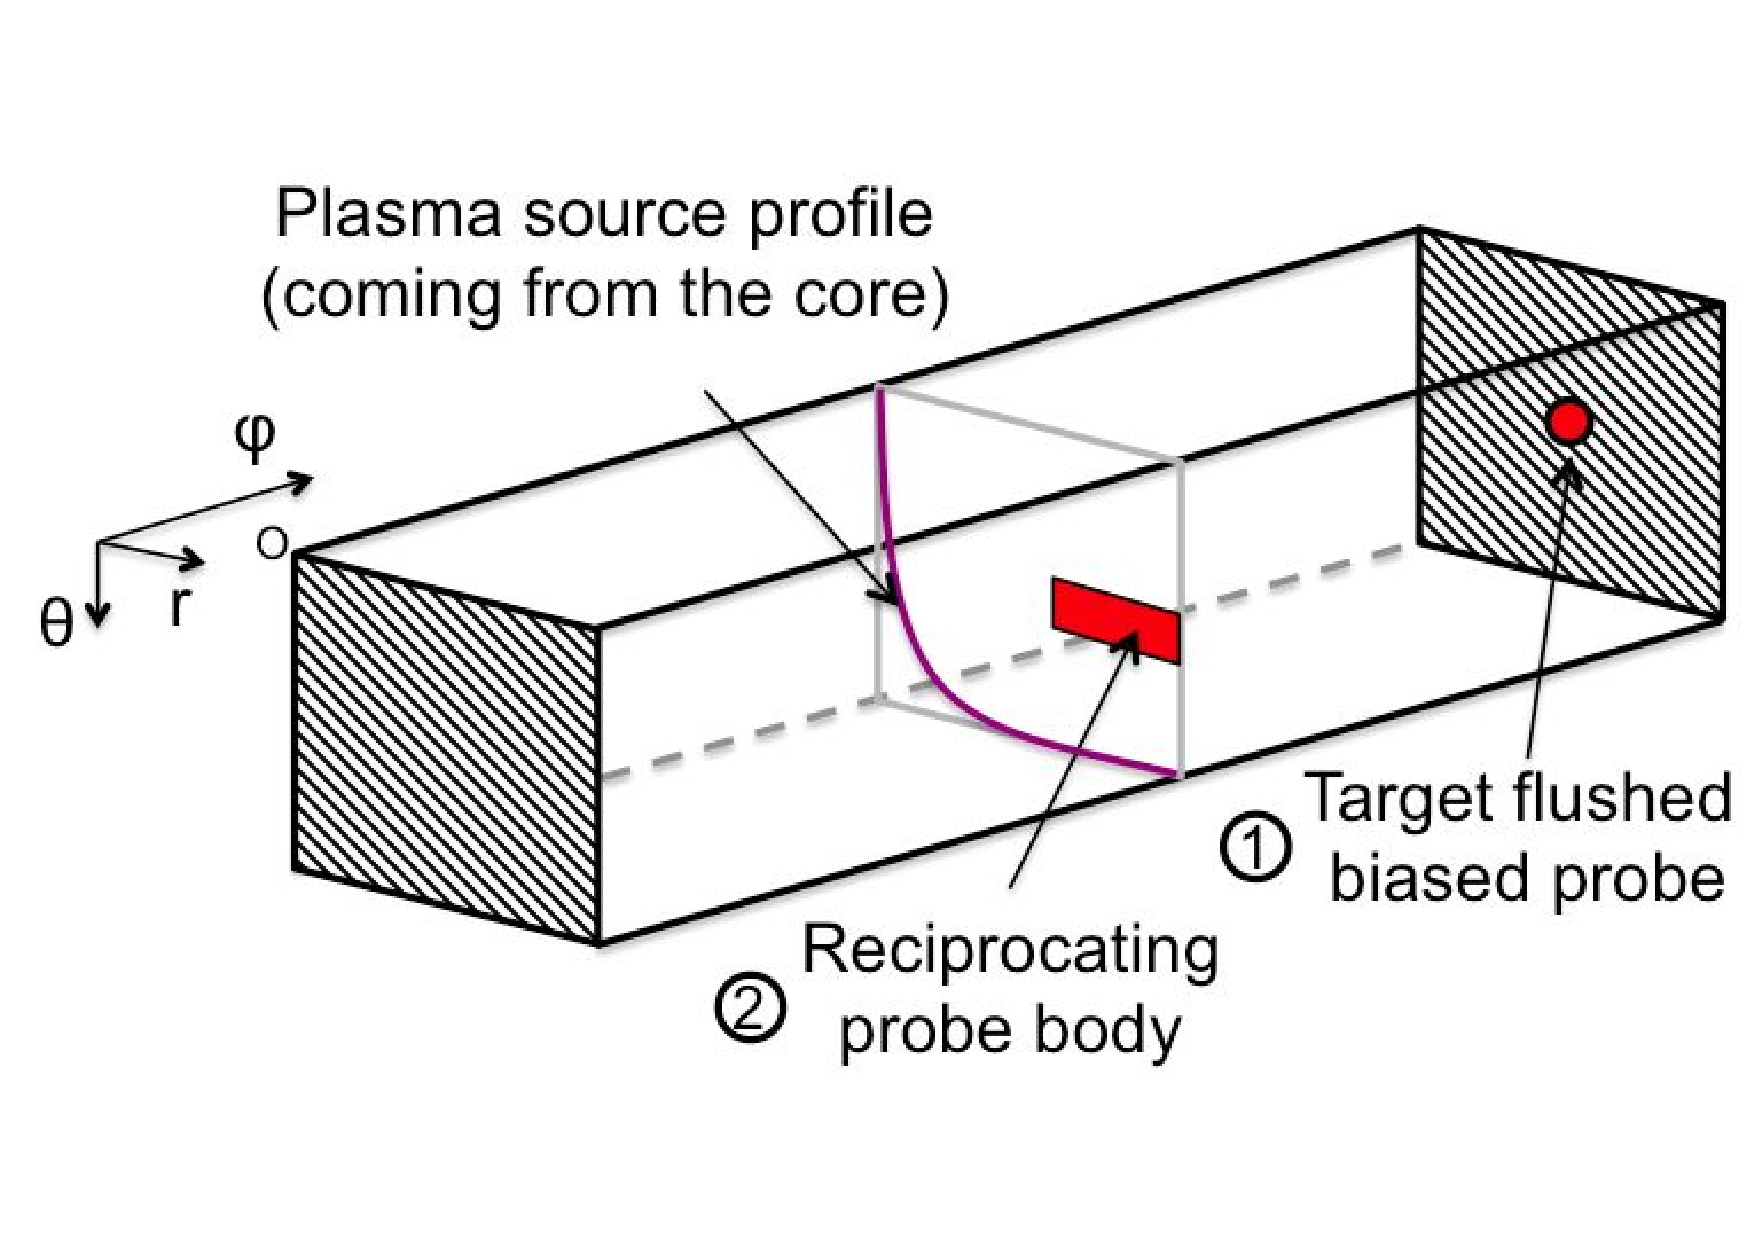
\includegraphics[width=\textwidth]{figures/geometry.pdf}
  \end{minipage}\hfill
  \begin{minipage}[c]{0.45\textwidth}
    \caption{Sketch of the slab geometry for the SOL. Divertor plates are 
 located at the end of the field lines, depicted with hatchings. The flushed
 probe is situated in the center of the top divertor plate and the mobile
 probe inserted in the middle of the domain. The
 profile of the source term driving the system is aslo roughly indicated for
 comprehension purposes.} \label{fig:1}
  \end{minipage}
\end{figure}

 The interaction between the probe
and the SOL plasma is described by the sheath theory in strong magnetic
fields, with field lines perpendicular to the wall~\cite{Bohm49}.
The flushed probe is then modeled by a local polarization of the target plates,
via a modification of the parallel Bohm boundary conditions :
 
 $$\Gamma_{\parallel\text{p}}=\pm
N_\text{p}\exp(\Lambda-\Phi_\text{p}+\Phi_\text{wall})
 \qquad
 J_{\parallel\text{p}} = \pm
 N_\text{p}(1-\exp(\Lambda-\Phi_\text{p}+\Phi_\text{wall}))
$$ 

$\Gamma_{\parallel\text{p}}$, $N_\text{p}$,
$\Phi_\text{p}$ and $J_{\parallel\text{p}}$ are plasma quantities in front of the
probe but still at the sheath entrance. The wall polarization
has a gaussian shape
$\Phi_\text{wall}=V_\text{p}\text{~}\exp(-(X-X_\text{p})^2/L_\text{p}^2)\text{~}\exp(-(Y-Y_\text{p})^2/L_\text{p}^2)$
with $V_\text{p}$ the applied bias voltage, $(X_\text{p}, Y_\text{p})$ the position and $L_\text{p}$ the
size of the probe. In the limit of strong negative polarization\footnote{with a
typical SOL electronic temperature $T_0\approx$ 100 eV, $V_\text{p}=-3$ corresponds to
approximately -300V}, the Boltzmann exponential term tend toward zero locally:
only ions reach the probe and the current drawn by the probe is
equal to the ion flux, ie. the probe is run on ion saturation mode.

On the other hand, the probe body is geometrically modelled by introducting
a solid obstacle with sheath boundary condition in the middle of the plasma. The
probe covers an area of 32 $\rho_L$ in the poloidal direction and occupies
radially the second half of the computationnal zone. In the parallel
direction the probe is infinitly thin, which seems reasonnable when
considering the size of the probe in comparison to the
parallel length $L_\parallel$ of the plasma.
At least, the probe body is taken conductive, but could just as well be chosen
insulating, as we will mostly focus on density and flux perturbations.

\section{Polarisation of the divertor probe}

As stated in previous works~\cite{Ghendrih03, Colin14, Futtersack16}, the
Langmuir probe in ion saturation mode impacts the surrounding plasma and could give
measurements leading to an underestimation of the plasma quantities. 
An illustration of the perturbation is given in Fig.~\ref{fig:2} :
 the parallel current drawn by the probe is maximum at the front of the probe, decreasing 
along and spreading across the magnetic field lines. We can also 
observe close to the probe the area of the return current which extends 
non-symetricaly along the radial direction on approximately one probe 
size $L_p$. Following 
the Ohms law Eq.~\eqref{eq_Ohms_law}, the parallel current has to come from a parallel gradient 
of potential and thus requires that the plasma in front of the probe stays at a different 
potential than the one of the unperturbed plasma. The perpendicular
electric field which rises then gives birth to an ExB vortex around all the flux tube,
preventing the turbulent plasma to reach the probe tip. To study
this phenomon, we define $\Psi=\Lambda-\Phi_\text{p}$, the difference of potential between 
the front of the probe and the unperturbed plasma, which characterizes the magnitude of the 
perturbation and thus the strengh of the vortex. We also look at $l_\parallel$, the parallel 
extention of the perturbation.


\begin{figure}
\begin{minipage}{68mm}
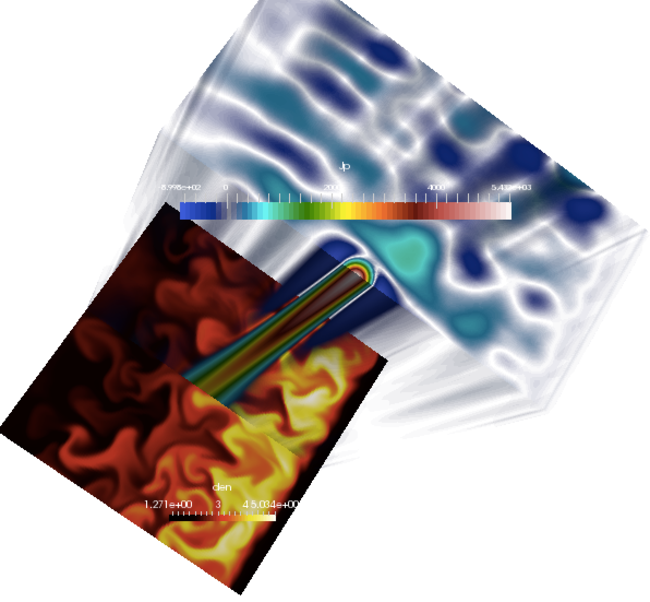
\includegraphics[width=\linewidth]{figures/3Dcurrent.pdf} \caption{3D view
of $J_\parallel$ from the top, where the probe is located. The white/transparent
color indicates zero current. The bottom plan shows the XY density map in strong
SOL electrostatic turbulence.}
\label{fig:2}
\end{minipage}
\hfill
\begin{minipage}{68mm}\vspace{20pt}
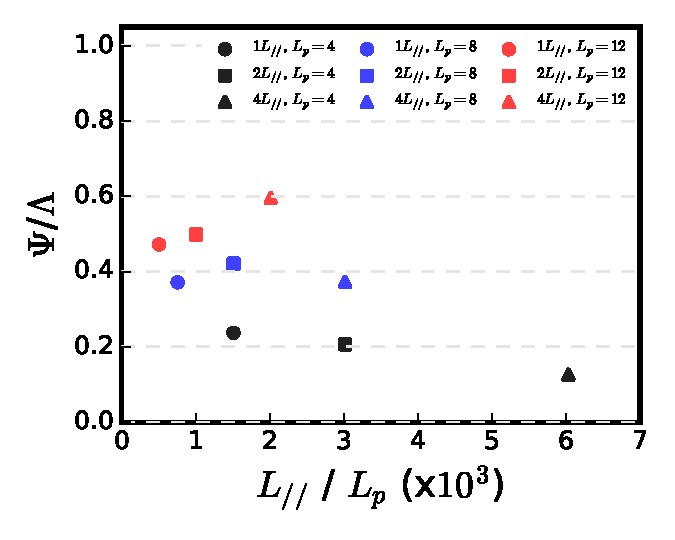
\includegraphics[width=\linewidth]{figures/perturbAmplLp.pdf}
\caption{Amplitude of the perturbation in front of the probe versus the ratio of the parallel 
to the probe lengths. Circles are for parallel length of 6x10$^3$, squares and triangles
are respectively for twice and fourth times the first $L_\parallel$. Colors show probes of the same sizes.}
\label{fig:3}

\end{minipage}
\end{figure}

In a semi-infinite plasma, the perturbation would extend along the field lines 
until the current transported across the magnetic field compensates the current drawn 
by the probe $J_{\parallel\text{p}}=l_\parallel \nabla_\perp\cdot \mathbf{J}_\perp $. Considering the turbulent perpendicular transport of 
current around the probe as an hyper-diffusif process $\mathbf J_\perp=-\nu_\text{turb}\nabla \nabla^2\Phi$ of perpendicular scale $L_\text{p}$,
 and combining this with Eq.~\eqref{eq_Ohms_law},
the parallel scale $l_\parallel$ of the perturbation can be estimated as :
\begin{equation}
\label{ExtensionPerturbation}
  l_{\parallel}=\sqrt{\frac{\eta^{-1}}{\nu_\text{turb}}}L_\text{p}^2
\end{equation}

Then, the integration of the current divergence equation along the parallel direction from the probe to $l_\parallel$
where the perturbation vanish and no parallel current exists let us express the amplitude of the perturbation
as :
\begin{equation}
\label{AmplitudePerturbation}
  \Psi\approx\sqrt{\frac{\eta}{\nu_\text{turb}}}L_\text{p}^2=
  l_\parallel \eta 
\end{equation}

Fig.~\ref{fig:3} shows the amplitude of the perturbation normalized to 
the floating potential as a function of the ratio 
$L_\parallel/L_\text{p}$. There is two immediate observations : the first 
one is that $\Psi$ does depend on the parallel length of the domain 
$L_\parallel$, in contradiction with the simple semi-infinite plasma 
assumption, where the perturbation should vanish at $l_\parallel \ll 
L_\parallel$. The second observation, which accords well to 
Eq.~\eqref{AmplitudePerturbation}, is that at a fixed $L_\parallel$, a larger 
probe will produce a larger perturbation. 

On another hand, we 
could have expected that increasing the parallel length would lead to weaken 
the perturbation as the perpendicular current would have been collected on a longer 
area. This is correct for the small probe $L_\text{p}$=4, but in 
contradiction with 
the results of the simulations for probes of size $L_\text{p}$=8 and 
$L_\text{p}$=12. This difference can however be explained when reconsidering 
the semi-infinite plasma hypothesys : as a matter of a fact, the SOL 
plasma takes its place between the two sides of the limiter/divertor 
separated in our simulations by a parallel length of 6x10$^3$ - 
2x10$^4$ (hence around 5m-20m, in a small tokamak with 
$T_e^\text{(SOL)}\approx$100eV). With a parallel resistivity $\eta$ of 
10$^{\text{ -5}}$, the parallel scale of the perturbation is of the same order 
or even exceed the parallel length of the system : 
$l_\parallel/L_\parallel\in$ [1,10]. The perturbaton reaches thus 
easily the opposite wall, drawing current directly from it. In this 
case, the probe IV characteristics should be interpreted as those of 
double probes. 

Supposing now that the total perpendicular current divergence is low enough 
(with a very short parallel length for example) to consider 
$\nabla_\parallel\cdot \mathbf j =0$ giving a parallel current constant 
all along the field line and equal to the saturation current drawn by 
the probe. Inserting in Eq.~\eqref{eq_Ohms_law} then gives :
\begin{equation}
\label{eqConstantCurrent2}
  j_\parallel=-\eta^{-1}\nabla_\parallel\Phi=j_\text{sat}\qquad\text{and thus}
  \qquad \Phi_\text{opp}-\Phi_\text{p}=L_\parallel\eta j_\text{sat}
\end{equation}

Moreover, as no curent comes from the perpenducular direction, the 
current drawn by the probe has to come entirely from the opposite wall. 
Expressing $\Phi_\text{opp}$ with the sheath theory and 
substituting the saturation currents, we can see that when the 
perpendicular current divergence is weak :
\begin{equation}
\label{eqConstantCurrent3}
  \Psi=\ln\left(
  1+\frac{N_\text{p}}{N_\text{opp}}\right)+L_\parallel\eta N_\text{p}
\end{equation}

In this situation, the perturbation in front of the probe grows when 
$L_\parallel$ increases. For a given probe size, two behaviours are 
then in competition depending on the total divergence 
of the perpendicular current, and there is a maximum of the amplitude 
of the perturbation at a specific $L_\parallel$, which can be seen on 
Fig.~\ref{fig:3} for the $L_\text{p}$=8 probe size.

Another way to look at $\Psi$, remember of 
Stangeby~\cite{Stangeby95-2}, is considering it as an adaptation to the 
probe voltage : indeed, rewriting the definition of $\Psi$ as 
$\Phi_\text{p}=\Lambda-\Psi=\Lambda-\alpha V_\text{p}$ let us define 
$\alpha=\Psi/V_\text{p}$, an accomodation factor of the plasma potential to the probe 
voltage, positive and even between zero and one. Then in sweeping 
operations to measure IV characteristics, if the plasma potential adapts to the probe voltage,
the elecron current drawn by the probe should also be affected :
\begin{equation}
J_{\parallel 
\text{p}}^e=N_\text{p}\exp\left(\Lambda-\Phi_\text{p}+V_\text{p}\right)=
N_\text{p}\exp\left(V_\text{p}(1-\alpha)\right)
\end{equation}

As a consequence, we see that if $\alpha$ differs significantly from 
zero, the measured slope on the IV characteristic, $T_e$,  
will always be overestimated, by the factor $(1-\alpha)^{-1}$. 
\vspace{2mm}
\begin{figure}
\begin{minipage}[c]{68mm}
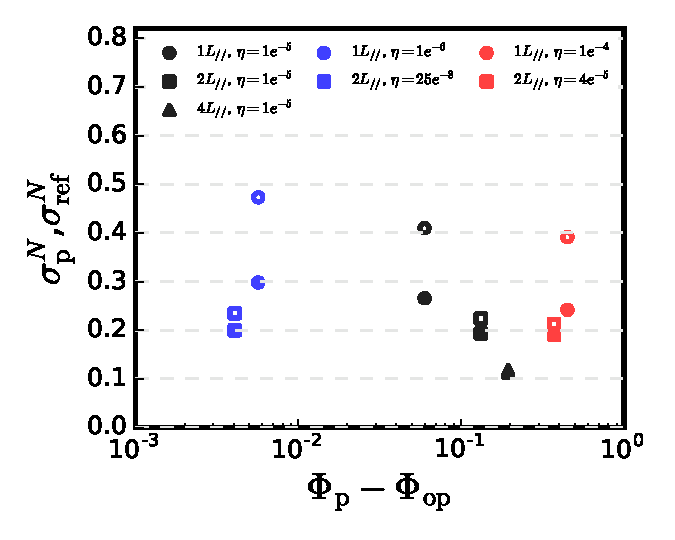
\includegraphics[width=68mm]{figures/perturbAmplEta.pdf}
\end{minipage}
\begin{minipage}[c]{\textwidth-68mm}
\caption{Standard deviations of density fluctuations in front of the 
probe (filled symbols) in comparison with the reference case (empty 
symbols) as a function of the 
potential difference between the walls. In blue on the left (small 
electric field), are the "conductive" cases with a low $\eta$. On the 
right (high electric field) are the "resistive" cases. Circles, squares 
and triangle are respectively for the base parallel length, times two 
and four.}
\label{fig:4}
\end{minipage}
\end{figure}

Let us look now at the effect of $\eta$ on the perturbation. When the 
probe is run in ion saturation mode, we are mostly interested by the 
density perturbation just in front of it. 
Eqs.~\eqref{ExtensionPerturbation}, \eqref{AmplitudePerturbation} and 
\eqref{eqConstantCurrent3} tell that increasing the resistivity should 
lead to a stronger perturbation, with a lower parallel extension. Also, 
when $l_\parallel$ is small enough, we can expect the transport 
barrier created by the vortex to act only on a part of the field line, and 
consequently that it exists a plasma refilling of the probe channel by 
parallel transport from the other side of the flux tube. On the 
contrary, if $l_\parallel$ is long in comparison to $L_\parallel$, the 
perturbation should be constant along the field line, reaching the 
opposite wall, and the vortex would prevent the plasma to enter the 
probe channel from either sides.
Less obvious on the mean plasma density, this effect is clear on the 
fluctuations levels, as showed on Fig.~\ref{fig:4}, from which we can 
extract two main trends :

\begin{enumerate}
\item Fluctuations are largely reduced in comparison to the unperturbed 
case, when the parallel length $L_\parallel$ is small, which is less 
evident when increasing the resistivity.
\item  Increasing the resistivity leads to a small reduction of $\sigma_N$ 
and $\sigma_\text{ref}$, but the principal effect is the increase of 
the parallel electric field.
\end{enumerate}

In the case of ITER, where the plasma will be hot and highly 
conductive, we can expect a strong connection of the perturbation 
between the two sides of the divertor. The flushed mounted probes 
should then act like double probes, the current being limited by the 
sheath of the opposite wall.

These results should nethertheless be significantly impacted by the 
plasma-neutrals interactions short-circuiting transverse 
transport of current and by the shear of the magnetic field impacing the shape of the probe flux tube.

\section{Reciprocating probe body and synthetic Mach measurements}


In this section, we study for the first time the impact of a probe 
body inserted in the SOL plasma with a full 3D turbulent code, at the 
scale of the Larmor radius. The geometry and the dimensions of the 
problem are sketched on Fig.~\ref{fig:1} of the model section. After a 
description of the main impacts of the probe on the SOL plasma 
characteristics, we will reconstruct and study a synthetic Mach probe 
measurement following the Hutchinson theory~\cite{Hutchinson02}.
\begin{figure}
\begin{minipage}{200mm}

\begin{minipage}{54mm}

\center\textbf{a)}\end{minipage}
\begin{minipage}{54mm}
\center\textbf{b)}\end{minipage}
\begin{minipage}{52mm}
\center\textbf{c)}\end{minipage}
\end{minipage}
 \begin{minipage}{52mm}
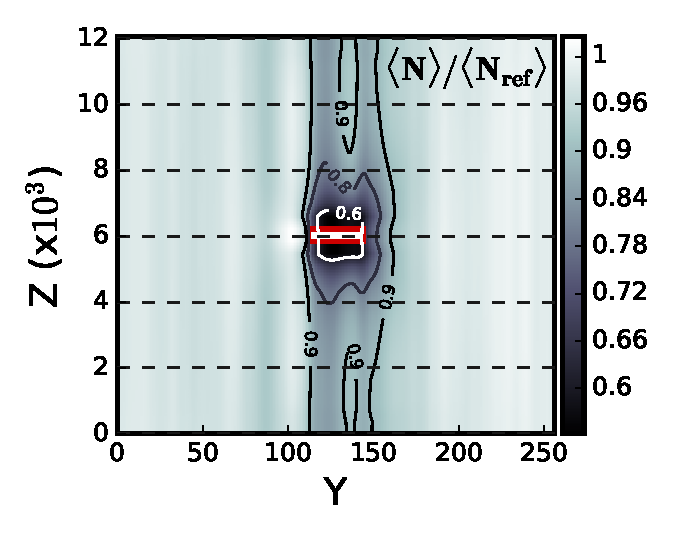
\includegraphics[width=52mm,trim = 0mm 0mm 0mm
0mm,clip]{figures/densityMapProbe.pdf}
\end{minipage}
 \begin{minipage}{52mm}
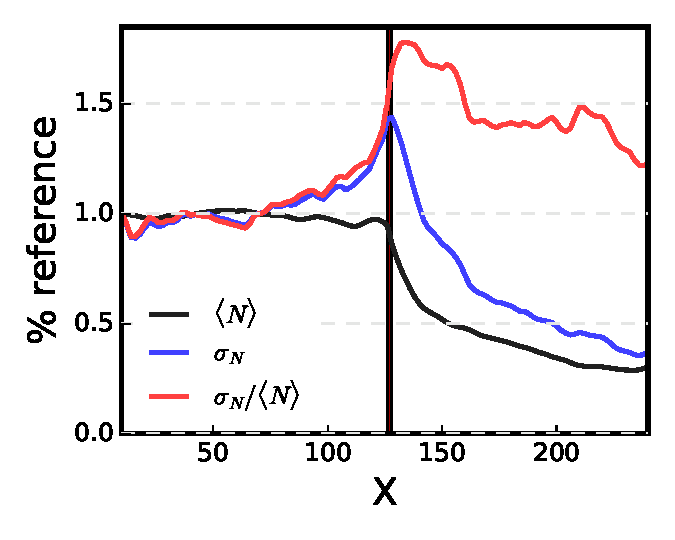
\includegraphics[width=52mm,trim = 0mm 0mm 0mm
0mm,clip]{figures/radialProfileProbe.pdf}
\end{minipage}
 \begin{minipage}{52mm}
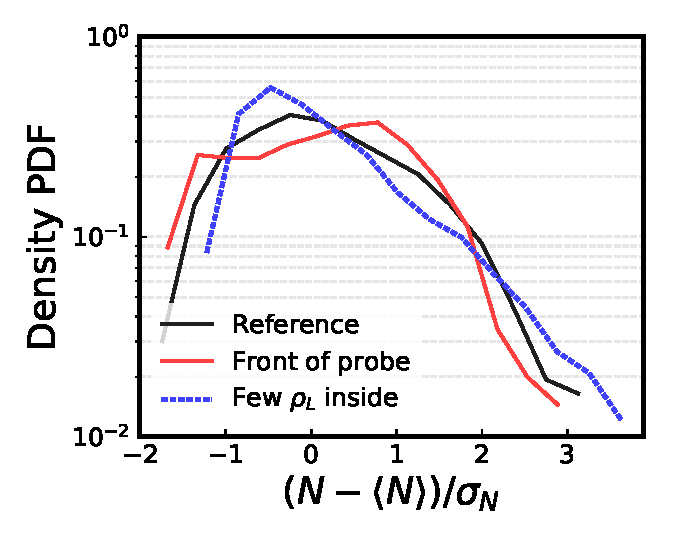
\includegraphics[width=52mm,trim = 0mm 0mm 0mm
0mm,clip]{figures/pdfProbe.pdf}
\end{minipage}
\begin{minipage}{\linewidth}
\caption{\textbf{a)}~Probe shadow in the poloidal plane. Map of the 
mean plasma density in comparison with the unperturbed 
case around the probe. The probe, in white, is situated at the middle of the field 
lines.
\textbf{b)}~Radial profile of the mean density, standard deviations and 
standard deviation normalized to $\left<N\right>$, rapported to the 
unperturbed reference case. The black line denotes the contact point 
with the probe.
\textbf{c)}~PDFs of density for the reference case, just in front of 
the probe and few Larmor radius inside the probe shadow.}
 \label{fig:5}
  \end{minipage}
\end{figure}
\subsection{\bf Perturbation the SOL plasma due to the probe body}

The first principal effect of the insertion into the SOL of a solid 
object is the creation of its own secondary pre-sheaths, the object's 
shadow~\cite{Hutchinson91}. Indeed, as the length of the field 
lines is divided by two and the loss surface for the plasma doubles, it will 
exist, on the both side of the probe, two areas of reduced density, 
where the radial decay length is strongly shortened. 
This effect is clearly recovered in the simulations, as we can see on 
the Figs.~\ref{fig:5} : the shadow of the probe extends along all the 
field lines, the plasma density is depleted in the probe shadow, 
from 20\% to more than 40\%, and this just few $\rho_L$ after the first contact between the 
plasma and the probe. 
The plasma potential, which responds to the plasma pressure accordingly 
to the Boltzmann relation, is also deeply impacted : the potential 
difference which emerges between the unperturbed plasma and the 
probe shadow gives birth to perpendicular electric fields, radials along 
 the borders of the probe and poloidal in front of it. As in the 
 flushed probe cases, this perpendicular electric field creates 
strong transport barriers all around the shadow, accentuating the 
plasma depletion.

These two effects, namely the dump of plasma density due to presence 
of the probe and the transport barriers, both impact the plasma 
fluctuations inside the probe shadow, either by "reducing" the 
frequency of bursts and also by increasing their relative importance in 
comparison to $\left<N\right>$. In front of the probe, where the 
poloidal transport barrier emerges, the PDF shows that there is much 
more middle or mixed events, corresponding to avalanches stopped and 
redirected. More inside the probe shadow, we clearly observe a 
modification of the kurtosis of the PDF indicating less frequent but 
more important events. They correspond to the avalanches which pass 
through the barrier, with a density relatively much more important than 
the plasma in the probe shadow.

In this simple case, without parallel or poloidal mean flows, it should 
be 

\subsection{\bf Synthetic Mach measurements}
Measurements of plasma flow velocity are of prime importance in 
tokamaks and so far, Mach probes, or so called "Janus" probes, are the 
principal diagostics used in this objective. The principle of these 
probes is to measure the ion fluxes parallel to the magnetic field on 
both sides of the probe, the ratio of the 
fluxes giving then the Mach number of the flow. The theory, a 
one-dimentional model first developped 
by Stangeby\cite{Stangeby84} and refined by 
Hutchinson\cite{Hutchinson87,Hutchinson88,Hutchinson91}, is based on 
the following equations :
\begin{gather}
\nabla_\parallel\Gamma=-\nabla_\perp\cdot\left(N\mathbf 
V_\perp\right)
\\
\nabla_\parallel\left(\Gamma^2/N\right)+2\nabla_\parallel N= 
-\nabla_\perp\cdot\left(\Gamma\mathbf 
V_\perp\right)+\eta_H\nabla_\perp^2 M
\end{gather}

with the symbols defined according to 
\eqref{eq_particle_balance}-\eqref{eq_charge_balance}, $\mathbf V_\perp$ 
being the normalized perpendicular velocity, $M=\Gamma/N$ the parallel 
velocity normalized by the Bohm velocity, \emph{i.e.} the Mach number and 
$\eta_H$, the shear viscosity, introduced by Hutchinson, which is the term 
differencing fundamentaly his model from the one of Stangeby. 

The essence of this one-dimentional approximation is to consider the 
perpendicular divergence of fluxes as sources of matter and momentum :
\begin{gather}
S_N=-\nabla_\perp\cdot\left(N\mathbf V_\perp\right)
\\
S_\Gamma=-\nabla_\perp\cdot\left(\Gamma\mathbf 
V_\perp\right)-M\nabla_\parallel \left(NM\right)+\eta_H\nabla_\perp^2\Gamma/N
\end{gather}

For the particle source, Stangeby use either $S_N=\text{cste.}$ or 
$S_N\propto N$ while Hutchinson prefers to use a source deriving from a 
diffusive particle flux $S_N=D_\perp\left(N_\infty-N\right)/a^2$, with a 
unperturbed plasma density $N_\infty$ and $a$ the characteric perpendicular 
length of the probe. 
About the momentum source, that Hutchinson resumes as~\cite{Hutchinson02}:
\begin{gather}
S_\Gamma=\frac{D_\perp}{a^2c_s}\left(M_\infty-M\right)\left(N_\infty-N\left(1-
\alpha\right)\right)\qquad \text{with}\qquad\alpha=\eta_H/N D_\perp
\\
S_\Gamma=\frac{D_\perp}{a^2c_s}\left(M_\infty-M\right)\left(N_\infty\left(1+\alpha\right)-N
\right)\qquad \text{with}\qquad\alpha=\eta_H/ N_\infty D_\perp
\end{gather}

the inviscid case of Stangeby is recovered with by $\alpha=0$ and 
$S_\Gamma$ reduces to 
$S_N\left(M_\infty-M \right)$, representing the change in 
momentum of the flow in the flux tube due to the entrance of ions with 
the unperturbed velocity $M_\infty$. These two approaches give 
for Stangeby and Hutchinson respectively the following ratio of 
upstream to downstream fluxes : $R=(2+M_\infty)/(2-M_\infty)$ and 
$R=\exp\left(M_\infty/M_c\right)$, the value of the calibration factor 
$M_c$, resulting from a fit of models results, being 
situated between 0.41 (1D model) and 0.45 (2D). Hutchinson also remarks 
that in their experiment, Harbour and Proudfoot~\cite{Harbour84} fit this 
ratio with $M_c$ = 0.6, which could correspond to an $\alpha$ = 0.1 situation.

\begin{figure}
\begin{minipage}[c]{68mm}
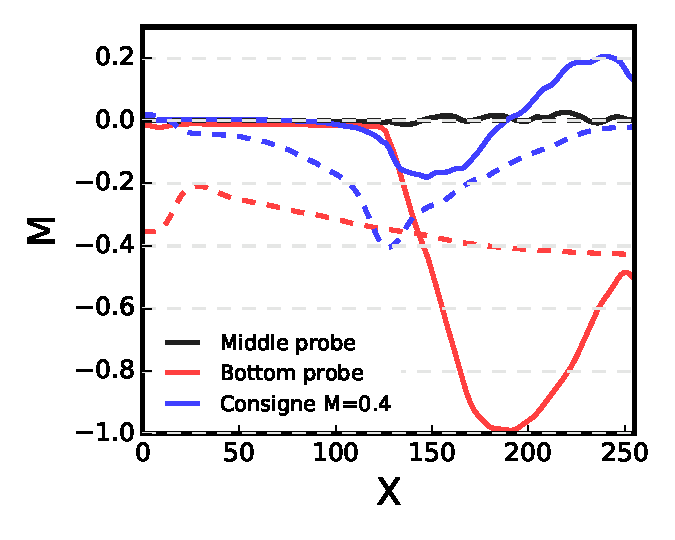
\includegraphics[width=68mm]{figures/hutchMachRadialProf.pdf}
\end{minipage}
\begin{minipage}[c]{\textwidth-68mm}
\caption{Synthetic measurement of flow Mach number following both 
formulas of Stangeby (dotted lines) and Hutchinson (dashed lines) and 
for three test cases : Black lines for the probe situated in the middle of the 
computational domain at $Z=L_\parallel/2$ with zero imposed parallel 
flow. Red Lines for a probe 
positioned at $Z=L_\parallel/4$ also without external parallel flow. 
Blue lines for the probe situated at $Z=L_\parallel/2$ but with an 
$M$ = 0.4 imposed external flow velocity.}
\label{fig:6}
\end{minipage}
\end{figure}

We reproduce these two measurements in figure~\ref{fig:6} for 
three different cases. The first one, where the probe is situated at 
the middle of the domain and without any parallel flow, measure the 
same density on each side of the probe (as the geometry is symmetric) 
and thus a correct parallel flow of $M_\infty$ = 0 for the both models.
In the second case, where the probe is situated at the bottom of the 
computation area, we can see that the measured Mach number, for the two 
models, varies between 0 and -1.5 along the radial direction. The both 
measurements give nethertheless the right value of $M_\infty\approx$ 0.4 
at a radial distance from the probe tip of respectively 6 (Stangeby) 
and 15 (Hutchinson with $M_c$ = 0.45).
In the third case, the probe is back to the center of the field lines, 
but we impose an external flow Mach number $M_\infty$ = 0.4 at the probe 
tip. Again, both measurements depends on the radial positition, but as 
the formula given by Stangeby give the right value at $X-X_p$ = 8, the 
model of Hutchinson underestimate everywhere the flux velocity.
At least, the both methods depend on the positioning of the probes on 
the probe body. If Stangeby's seems more accurate in our model of 
turbulent perpendicular transport, Hutchinson measurement can be calibrated 
with $M_c$. It is then worth to say that $M_c$ should be 
specific of a probe design and that none value could be 
used universaly.

Finaly, it should be pointed out that in the case of an uncentered probe, 
the density difference may not be only due to the probe wake. 
Indeed, if we modelize the perpendicular transport by a constant 
diffusion of coefficient $D_\perp$, the presheath equilibrium is 
reached when :
\begin{equation}
\nabla_\parallel \Gamma=D_\perp\nabla_\perp^2 N
\end{equation}
resulting in an radial profile exponentialy deacreasing for the 
density, whose decay length $\lambda_\text{SOL}$ defines the size of the SOL :
\begin{equation}
\lambda_\text{SOL}=\sqrt{\frac{D_\perp L_\parallel}{c_s}}
\end{equation}
With a probe separating the SOL presheath of parallel length 
$L_\parallel$ in two smaller presheaths of different length, saying 
$L_\parallel'$ and $L_\parallel''$, it is obvsious that the both decay 
lengths, and thus the density profiles on the two sides of the probes 
will differ significantly, even when $M_\infty=0$.

\begin{figure}
\begin{minipage}{68mm}
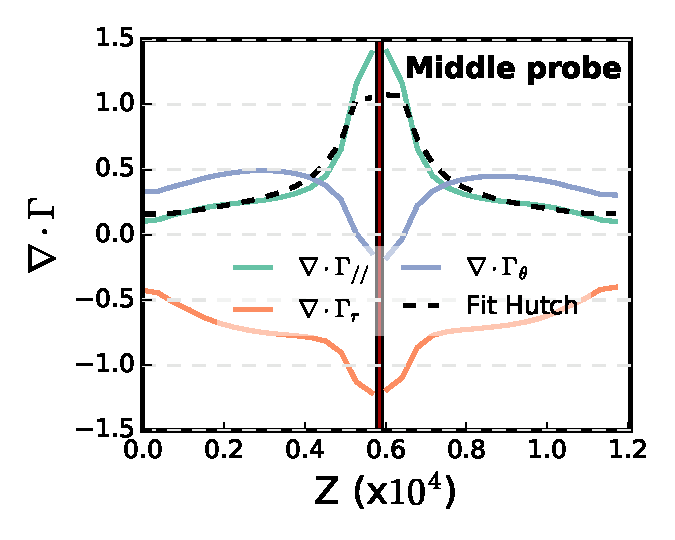
\includegraphics[width=\linewidth]{figures/PartBalance_middle.pdf} 
\caption{caption1}
\label{fig:7}
\end{minipage}
\hfill
\begin{minipage}{68mm}\vspace{20pt}
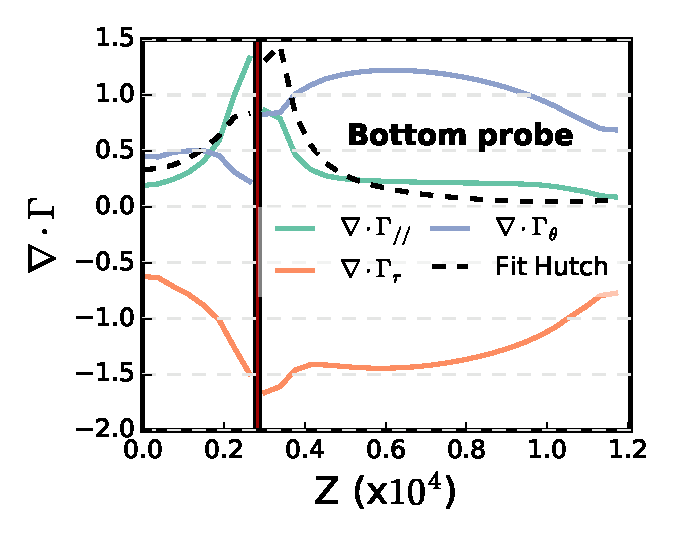
\includegraphics[width=\linewidth]{figures/PartBalance_bottom.pdf}
\caption{caption2}
\label{fig:8}


\end{minipage}
\end{figure}
\begin{figure}
\begin{minipage}{68mm}
\includegraphics[width=\linewidth]{figures/MomentumBalance_middle.pdf} 
\caption{caption3}
\label{fig:9}
\end{minipage}
\hfill
\begin{minipage}{68mm}\vspace{20pt}
\includegraphics[width=\linewidth]{figures/MomentumBalance_bottom.pdf}
\caption{caption4}
\label{fig:10}

\end{minipage}
\end{figure}

\section{Conclusion}
% When the probe draws a current, some part has to come from the perpendicular
% direction\footnote{If the probe draws no current from the perpendicular
% direction, $\nabla_\parallel j_\parallel$ should be null, and thus $j_\parallel$
% a constant. The Bohm sheath conditions impose then $V_p=0$, and a zero parallel
% current as well.}. Let's assume a simple diffusive/viscous process controled by
% $\nu^*$.
% The charge balance equation gives
% 	$\nabla_\parallel j_\parallel=\nabla_\perp\cdot\nu^*\nabla_\perp\nabla_\perp^2
% 	\Phi$. If we suppose a mean perturbation on the potential of size $L_s$, the
% 	current equilibrium of the 2D model is then :
% 	\begin{gather}
% 	\sigma_\parallel(\Lambda-(\Phi-V_p)/T_p)=(\Phi-\Lambda
% 	T)\nu^*/L_s^2L_\perp^2\Longleftrightarrow\Phi\approx\frac{1}{1+r}\left(V_p-\Lambda\left(T+rT_p\right)
% 	\right)
% 	\end{gather}
% with $r=\nu /L_s^2L_\perp^2\sigma_\parallel$ a transport ratio. As $r\propto
% L_S^{-2}$, when the probe size increase, the plasma potential will adapt to the wall sheath
% potential $V_p-\Lambda T_p$, $T_p$ being the electronic temperature at the probe
% location. In contrast, for a small probe size of when the perpendicular
% transport is efficient, the plasma potential will go as the unperturbed plasma
% sheath potential $\Phi=\Lambda T$. The same work for the 3D case give , 

\begin{acknowledgement}
This work has been financialy supported by the French National Research
Agency through project ANR-11-BS09-023 (SEDIBA). It has been carried out within
the framework of the EUROfusion Consortium with a funding from the
Euratom research and training programme 2014-2018 in the frame of project
WP14-ER-01/CEA-09. The views and opinions expressed herein do not necessarily
reflect those of the European Commission. This work was granted access to the
HPC resources of Aix-Marseille Universit\'e financed by the project Equip@Meso
(ANR-10-EQPX-29-01) of the programme "Investissements d'Avenir" supervised by
the Agence Nationale pour la Recherche. It also used HPC resources from
GENCI-IDRIS in the frame of project i2015056912.
\end{acknowledgement}


\def\bstname{cpp}

 \bibliographystyle{cpp}
 \bibliography{biblio.bib}
% 
% Replace the following example bibliography with your references
% before submission:
%\providecommand{\WileyBibTextsc}{}
%\let\textsc\WileyBibTextsc
%\providecommand{\othercit}{}
%\providecommand{\jr}[1]{#1}
%\providecommand{\etal}{~et~al.}


%\begin{thebibliography}{[10]}


%\end{thebibliography}


\end{document}
